\documentclass[tikz,border=5pt]{standalone}
\usepackage{tikz}

\begin{document}
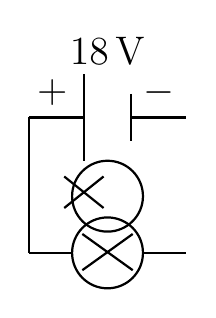
\begin{tikzpicture}[line width=0.8pt]

% --- Coordonnées principales ---
\def\yTop{2}
\def\yBot{0.28}
\def\xLeft{3}
\def\xRight{5}

% --- Fil de gauche ---
\draw (\xLeft,\yTop) -- (\xLeft,\yBot);

% --- Fil du haut avec pile ---
\draw (\xLeft,\yTop) -- (3.7,\yTop);

% Pile
\draw (3.7,\yTop+0.55) -- (3.7,\yTop-0.55); % grande borne
\draw (4.3,\yTop+0.30) -- (4.3,\yTop-0.30); % petite borne

% Suite du fil du haut
\draw (4.3,\yTop) -- (\xRight,\yTop);

% --- Interrupteur fermé à droite ---
% petit fil vertical au-dessus


% contacts



% petit fil vertical au-dessous

% --- Fil du bas avec ampoule ---
\draw (\xLeft,\yBot) -- (3.55,\yBot);
\draw (4.45,\yBot) -- (\xRight,\yBot);

% Ampoule
\draw (4,\yBot) circle (0.45);
\draw (3.68,0.52) -- (4.32,0.06);
\draw (3.68,0.06) -- (4.32,0.52);

\draw (4.00,1.00) circle (0.45);
\draw (3.45,1.25) -- (3.95,0.85);
\draw (3.45,0.85) -- (3.95,1.25);

% --- Étiquettes de la pile ---
\node at (4.00,2.85) {\Large $18\,\mathrm{V}$};
\node at (3.30,2.32) {\Large $+$};
\node at (4.65,2.32) {\Large $-$};

\end{tikzpicture}
\end{document}